\documentclass{paper}

\usepackage{amsmath,lstautogobble,amssymb,amsfonts, listings, fancyhdr, stmaryrd, array, tikz}
\usepackage[many]{tcolorbox}
\usepackage[T1]{fontenc}
\usepackage[utf8]{inputenc}
\usepackage[a4paper, total={170mm,257mm}, left=20mm, top=20mm]{geometry}
\usepackage{adjustbox}
\definecolor{color0}{HTML}{000000}
\definecolor{color1}{HTML}{000000}
\definecolor{bgColor}{HTML}{ffffff}
\usetikzlibrary {arrows.meta,bending} 

\newtheorem{proposition}{Proposition}
\newtheorem{definition}{Definition}
\newtheorem{preuve}{Preuve}

\definecolor{codegreen}{rgb}{0,0.6,0}
\definecolor{codegray}{rgb}{0.5,0.5,0.5}
\definecolor{codepurple}{rgb}{0.58,0,0.82}
\definecolor{backcolour}{rgb}{0.95,0.95,0.92}
\lstdefinestyle{mystyle}{
    language=caml,
    backgroundcolor=\color{backcolour},   
    commentstyle=\color{codegreen},
    keywordstyle=\color{magenta},
    numberstyle=\tiny\color{codegray},
    stringstyle=\color{codepurple},
    basicstyle=\ttfamily\footnotesize,
    breakatwhitespace=false,         
    breaklines=true,                 
    captionpos=b,                    
    keepspaces=true,                 
    numbers=left,                    
    numbersep=5pt,                  
    showspaces=false,                
    showstringspaces=false,
    showtabs=false,                  
    tabsize=2,
    autogobble=true
}

\lstset{style=mystyle}

\newcolumntype{C}{>$c<$}
\tcolorboxenvironment{proposition}{enhanced, borderline={0.8pt}{0pt}{blue}, borderline={0.4pt}{2pt}{cyan}, boxrule=0.4pt, colback=white, coltitle=black, sharp corners}
\tcolorboxenvironment{definition}{ enhanced, borderline={0.8pt}{0pt}{red}, borderline={0.4pt}{2pt}{orange}, boxrule=0.4pt, colback=white, coltitle=black, sharp corners}
\tcolorboxenvironment{preuve}{ enhanced, borderline={0.8pt}{0pt}{green}, borderline={0.4pt}{2pt}{lime}, boxrule=0.4pt, colback=white, coltitle=black, sharp corners}

\pagestyle{fancy}
\fancyhead[C]{TIPE-ENS Rapport - Dorian GIL}

\begin{document}
\setlength{\headheight}{13.07225pt}
\addtolength{\topmargin}{-1.07225pt}

\section*{Etude d'un algorithme de vérification de modèle en Logique Linéaire Temporelle}

Dans un monde dont la dépendance à divers technologies est très importante, il est important de s'assurer du bon fonctionnement de ces technologies.
C'est ainsi que la vérification de modèle rentre en jeu pour répondre à ces problèmatiques. Ce sont des techniques de vérifications qui explorent tout les 
états possible d'un système de manière force brute. Nous allons donc étudier une famille d'algorithme permettant de résoudre de tel problème.






\section{Préliminaires}

\subsection{Logique Linéaire Temporelle}

    \begin{definition}[Formule de la LTL]
        On définit les opérateurs suivants:
            \begin{itemize}
                \item $X\phi$ : $\phi$ doit être satisfaite dans l'état suivant (neXt)
                \item $\psi U\phi$ : $\psi$ doit être satisfaite dans tous les états jusqu'à un état où $\phi$ est satisfait (Until)
                \item $F\phi$ : $\phi$ doit être satisfaite une fois plus tard (Finally)
                \item $G\phi$ : $\psi$ doit être satisfaite dans tous les états futurs (Globally)
            \end{itemize}
        On définit $F$ l'ensemble des formules de la LTL inductivement par:
        \begin{itemize}
            \item $p\in AP \implies p\in F$
            \item si $\psi$ et $\phi$ sont des formules de LTL alors $\lnot\psi, \phi\lor\psi, \textbf{X}\psi, \phi \textbf{U}\psi$ sont des formules de LTL
        \end{itemize}
        $AP$ un ensemble fini de variables propositionnelles.
    \end{definition}

    Soit $v : \omega\times F \rightarrow \{T,F\}$ une fonction de valuation.
    
    \begin{definition}[Monde]
        On définit un tel objet comme $\omega := w_0,w_1,\dots$ une suite infinie d'état.
        On écrira $\omega^i:=w_i,w_{i+1},\dots$ un suffixe de $\omega$.
        On définit $\omega \models f$ via:
        \begin{itemize}
            \item $\omega \models a \Leftrightarrow v(w_0,a) = T$ si $a$ atomique 
            \item $\omega \models \lnot f$ si $\lnot(\omega \models f)$ 
            \item $\omega \models f\lor g$ si $\omega \models f$ ou $\omega \models g$
            \item $\omega \models \textbf{X}f$ si $\omega^1 \models f$
            \item $\omega \models f\textbf{U}g$ si $\omega \models g$ ou $\omega \models f\land\textbf{X}(f\textbf{U}g)$
            \item $\omega \models \textbf{F}f$ si $\exists i, \omega^i \models f$
            \item $\omega \models \textbf{G}f$ si $\forall i, \omega^i \models f$
        \end{itemize}
    \end{definition}





\subsection{Méthode des tableaux}

    \begin{definition}[Méthode des tableaux]
        Algorithme pour prouver qu'une assertion $\phi$ ayant pour hypothèse $(H_n)$ soit satisfiable. En bref:
        \begin{itemize}
        \item On place $\phi$ et ses hypothèses dans la racine.
        \item On applique des règles $(R_x)$ à chaque formule en bout d'arbre qui sont developpables
        \item Si on trouve des contradictions (des \textit{cycles}) dans toutes les branches de l'arbre (branches fermées), l'arbre est fermé donc la formule est insatisfiable.
        \end{itemize}
    \end{definition}

    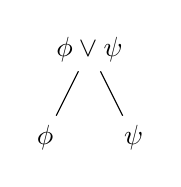
\begin{tikzpicture}[scale=0.75]
    \node {$\phi\lor\psi$}
        child {node {$\phi$}}
        child {node {$\psi$}};
    \end{tikzpicture}
    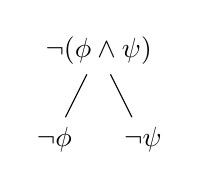
\begin{tikzpicture}[scale=0.75]
    \node {$\lnot(\phi\land\psi)$}
        child {node {$\lnot\phi$}}
        child {node {$\lnot\psi$}};
    \end{tikzpicture}
    \begin{tikzpicture}[scale=0.75]
    \node {$\lnot\lnot\phi$}
        child {node {$\phi$}};
    \end{tikzpicture}
    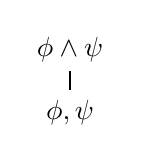
\begin{tikzpicture}[level distance=8mm]
    \node {$\phi\land\psi$}
        child {node {$\phi, \psi$}};
    \end{tikzpicture}  
    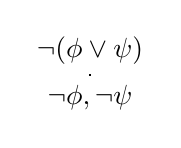
\begin{tikzpicture}[level distance=8mm,scale=0.75]
    \node {$\lnot(\phi\lor\psi)$}
        child {node {$\lnot\phi, \lnot\psi$}};
   \end{tikzpicture}

    On définit deux nouvelles règles pour la méthode des tableaux en LTL:
    
    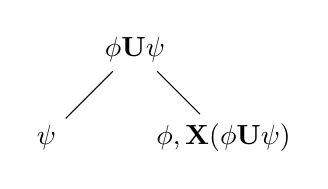
\begin{tikzpicture}[scale=0.75, level 1/.style={sibling distance=3cm}]
    \node {$\phi\textbf{U}\psi$}
        child {node {$\psi$}}
        child {node {$\phi, \textbf{X}(\phi\textbf{U}\psi)$}};
    \end{tikzpicture}
    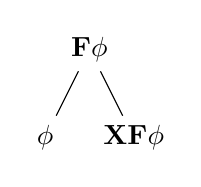
\begin{tikzpicture}[scale=0.75]
    \node {$\textbf{F}\phi$}
        child {node {$\phi$}}
        child {node {$\textbf{XF}\phi$}};
    \end{tikzpicture}
    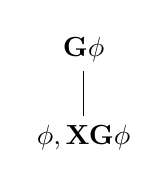
\begin{tikzpicture}[scale=0.75]
    \node{$\textbf{G}\phi$}
        child {node {$\phi, \textbf{XG}\phi$}};
    \end{tikzpicture}

    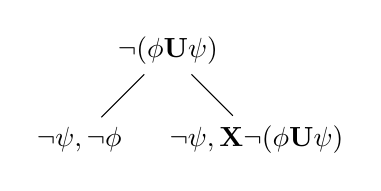
\begin{tikzpicture}[scale=0.75, level 1/.style={sibling distance=3cm}]
    \node {$\lnot(\phi\textbf{U}\psi)$}
        child {node {$\lnot\psi, \lnot\phi$}}
        child {node {$\lnot\psi, \textbf{X}\lnot(\phi\textbf{U}\psi)$}};
    \end{tikzpicture}
    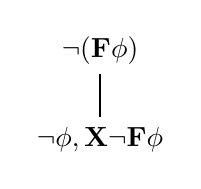
\begin{tikzpicture}[scale=0.75]
    \node {$\lnot(\textbf{F}\phi)$}
        child {node {$\lnot\phi, \textbf{X}\lnot\textbf{F}\phi$}};
    \end{tikzpicture}
    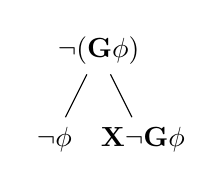
\begin{tikzpicture}[scale=0.75]
    \node {$\lnot(\textbf{G}\phi)$}
        child {node {$\lnot\phi$}}
        child {node {$\textbf{X}\lnot\textbf{G}\phi$}};
    \end{tikzpicture}

    En plus on rajoute des règles supplémentaires:  On appelle \textbf{X-eventualite} les formules de la forme $\textbf{X}(a\textbf{U}b)$ et $\textbf{XF}b$   
    On notera $x\leq y$ si $y$ est descendant de $x$ (resp < pour descendant strict)

    \begin{itemize}
        \item \textbf{LOOP:} Si un noeud $v$ a un ancètre strict $u$ tq $\Gamma_v \subseteq \Gamma_u$ et pour chaque $\textbf{X}(a\textbf{U}b)$ ou  $\textbf{XF}b$ dans $\Gamma_u$, il existe un noeud $w$ tq $b\in\Gamma_w$ et $u < w \leq v$ alors la formule de départ est satisfiable.
        \item \textbf{PRUNE:} Si $u < v < w$ et ont les mêmes hypothèses $\Gamma$ et que pour chaque $\textbf{X}(a\textbf{U}b)$ ou $\textbf{XF}b$ dans $\Gamma$, si on a $x$ tq $b\in\Gamma_x$ et $v < x \leq w$ alors $\exists y, b\in\Gamma_y$ et $u < y \leq v$ et $w$ ferme sa branche.
        \item \textbf{PRUNE$_0$:} Si $u < v$ et ont les mêmes hypothèses $\Gamma$ et que il y a au u moins une formule X-eventuelle, mais pas de formule de la forme $\textbf{X}(a\textbf{U}b)$ ou $\textbf{XF}b$ dans $\Gamma$ où $\exists x, b\in\Gamma_x$ et $u < x \leq v$ alors $v$ ferme sa branche.
        \item \textbf{TRANSITION:} Si aucune des autres règles ne s'applique, alors un noeud étiqueté par $\Gamma$ peut avoir un enfant dont l'étiquette est $\Delta = \{a | Xa\in\Gamma\}\bigcup\{\lnot a | \lnot Xa\in\Gamma\}$
    \end{itemize}

    \begin{proposition}[Correction et Complétude]
        La méthode des tableaux en logique linéaire temporelle est correct et complet
    \end{proposition}
    \begin{preuve}
        Par reccurrence immediate (non)
    \end{preuve}





\subsection{Automate de Buchi}

    \begin{definition}[Automate de Buchi (BA)]
        Un automate de Büchi est un 5-uplets $(S, I, T, F, \Sigma)$ tel que
        \begin{itemize}
            \item $S$ est un ensemble fini d'état
            \item $I\subseteq S$ un ensemble d'état initiaux
            \item $F\subseteq S$ un ensemble d'état finaux
            \item $\Sigma$ Un ensemble fini de symboles appelé alphabet
            \item $T: \{S\times \Sigma\}\mapsto \mathcal{P}(S)$ Une fonction de transition.
        \end{itemize}
        Cet automate particulier accepte des séquences infinis (donc des mots infinis) ssi le mot passe par un état acceptant une infinité de fois.
    \end{definition}

    \begin{proposition}[Test BA Vide]
        Un BA est non vide ssi il existe un état final qui est atteignable depuis un état initial et appartient à un cycle.
        
        \textbf{Algorithme:} On considère notre automate comme un graphe orienté, qu'on décompose en CFC, puis on fait un DFS depuis les etats initiaux et on trouve une CFC non trivial tq il contient un etat final et est atteignable par un état initial.
    \end{proposition}
    \begin{preuve}
    
    \end{preuve}
    
    \begin{definition}[Automate de Büchi généralisé (GBA)]
        C'est un automate de Büchi où on change l'ensemble des états finaux $F$ par $F_g\subseteq \mathcal{P}(S)$ appelé \textbf{condition d'acceptation}.
    \end{definition}
    Un GBA accepte un mot ssi il est passé une infinité de fois par un état dans chaque ensemble d'état acceptant.

    \begin{proposition}[GBA vers BA]
        Un ensemble multiple d'état acceptant peut être traduit en un ensemble en construisant un automate par une "counting construction". 
        C'est à dire si $A = (S,I, \{F_1,\dots,F_n\}, \Sigma, T)$, alors il est equivalent à $A' = (S',I', F, \Sigma, T')$ telle que
        \begin{itemize}
            \item $Q' = Q\times\{1,...,n\}$
            \item $I' = I\times\{1\}$
            \item $F'=F_1\times \{1\}$
            \item $\Delta' = \{ ( (q,i), a, (q',j) ) | (q,a,q') \in \Delta$ et si $q \in F_i$, $j= i+1 \mod n$ sinon $j=i \}$
        \end{itemize}
        qui est bien un automate de Büchi (non généralisé) qui accepte les mêmes mots.
    \end{proposition}
    \begin{preuve}
        
    \end{preuve}

\begin{proposition}[Intersection de BA]
    On définit l'automate reconnaissant l'intersection de deux langages comme $A'= (S', I', F', \Sigma, T')$ telle que
    \begin{itemize}
        \item $S'=S_1\times S_2\times \{1,2\}$
        \item $T'=T_1'\cup T_2'$
        \begin{itemize}
            \item $T_1=\{((q_1,q_2,1),a,(q_1',q_2',i)), (q_1,a,q_1')\in T_1, (q_2,a,q_2')\in T_2, q_1\in F_1 \Leftrightarrow i= 2, i\in[|1,2|]\}$
            \item $T_2=\{((q_1,q_2,2),a,(q_1',q_2',i)), (q_1,a,q_1')\in T_1, (q_2,a,q_2')\in T_2,  q_2\in F_2 \Leftrightarrow i= 1, i\in[|1,2|]\}$
        \end{itemize}
        \item $I'= I_1\times I_2 \times \{1\}$
        \item $F'= \{(q_1,q_2,2), q_2\in F_2 \}$
    \end{itemize}
    Il reconnait l'intersection des langages reconnues par les automates de Büchi
\end{proposition}
\begin{preuve}
    
\end{preuve}






\section{Résolution}

\subsection{Présentation}

    Pour résumé le déroulé de l'algorithme, nous devons faire en supposant l'implémentation de la méthode des tableaux en LTL faites et des automates de Büchi.
    
    \begin{enumerate}
        \item Création d'un automate $A_m$ correspondant au cahier des charges d'une technologies, sous forme des différents états dans lequel la technologie sera.
        \item Création d'un automate $A_{\lnot\varphi}$ où $\varphi$ représente les differentes contraintes que notre cahier des charges doit respecter, sous forme
        d'une formule logique en logique linéaire temporelle. 
        \item Création de l'automate Syncronisé $A_m\times A_{\lnot\varphi}$
        \item Si l'automate resultant est vide, alors c'est bon, sinon on renvoie un contre exemple.
    \end{enumerate}

    
    \textbf{Remarques:} 
    \begin{itemize}
        \item Nous supposerons l'étape 1 donné, l'étape 3 et 4 est immédiat par ce qu'on a définit en préliminaire.
        \item Intuitivement, Le langage des $A_m$ représente toutes les exécutions de $M$ et celui de $A_{\lnot\varphi}$ représente les exécutions ne satisfaisant pas la 
        formule $\varphi$. Le langage du produit est donc vide ssi tous les chemins de $M$ satisfont $\varphi$. Sinon il existe un mot en commun, qui nous donne l'erreur.
        \item Pour l'étape 1, en théorie l'automate est donné après transformation d'un système de transition $\mathcal{M}$ en un automate $A_{\mathcal{M}}$
    \end{itemize}



\subsection{Creation de $A_{\lnot\varphi}$}
    On présente ici l'algorithme de Gerth

\end{document}